\subsection{Leaflet for teams}

\begin{figure}[H]
	\begin{minipage}{0.3\linewidth}
		Nikita Safronov\\
		\emph{Role in team: captain, reserve drive-operator, responsible for writing the technical book, responsible for elevator and winch.\\}
		\emph{Information: 17 years old, in robotics 4 years, in FTC 2 years.\\} 
		\emph{Why I chose FTC: "I have chosen FIRST because I enjoy working with mechanisms and finding unusual technical decisions for solving problems. Also working on this project helps me to get new skills in a sphere of engineering. In this case I know, that I don't spend my time in vain."}				
	\end{minipage}
	\hfill
	\begin{minipage}{0.3\linewidth}
		\center{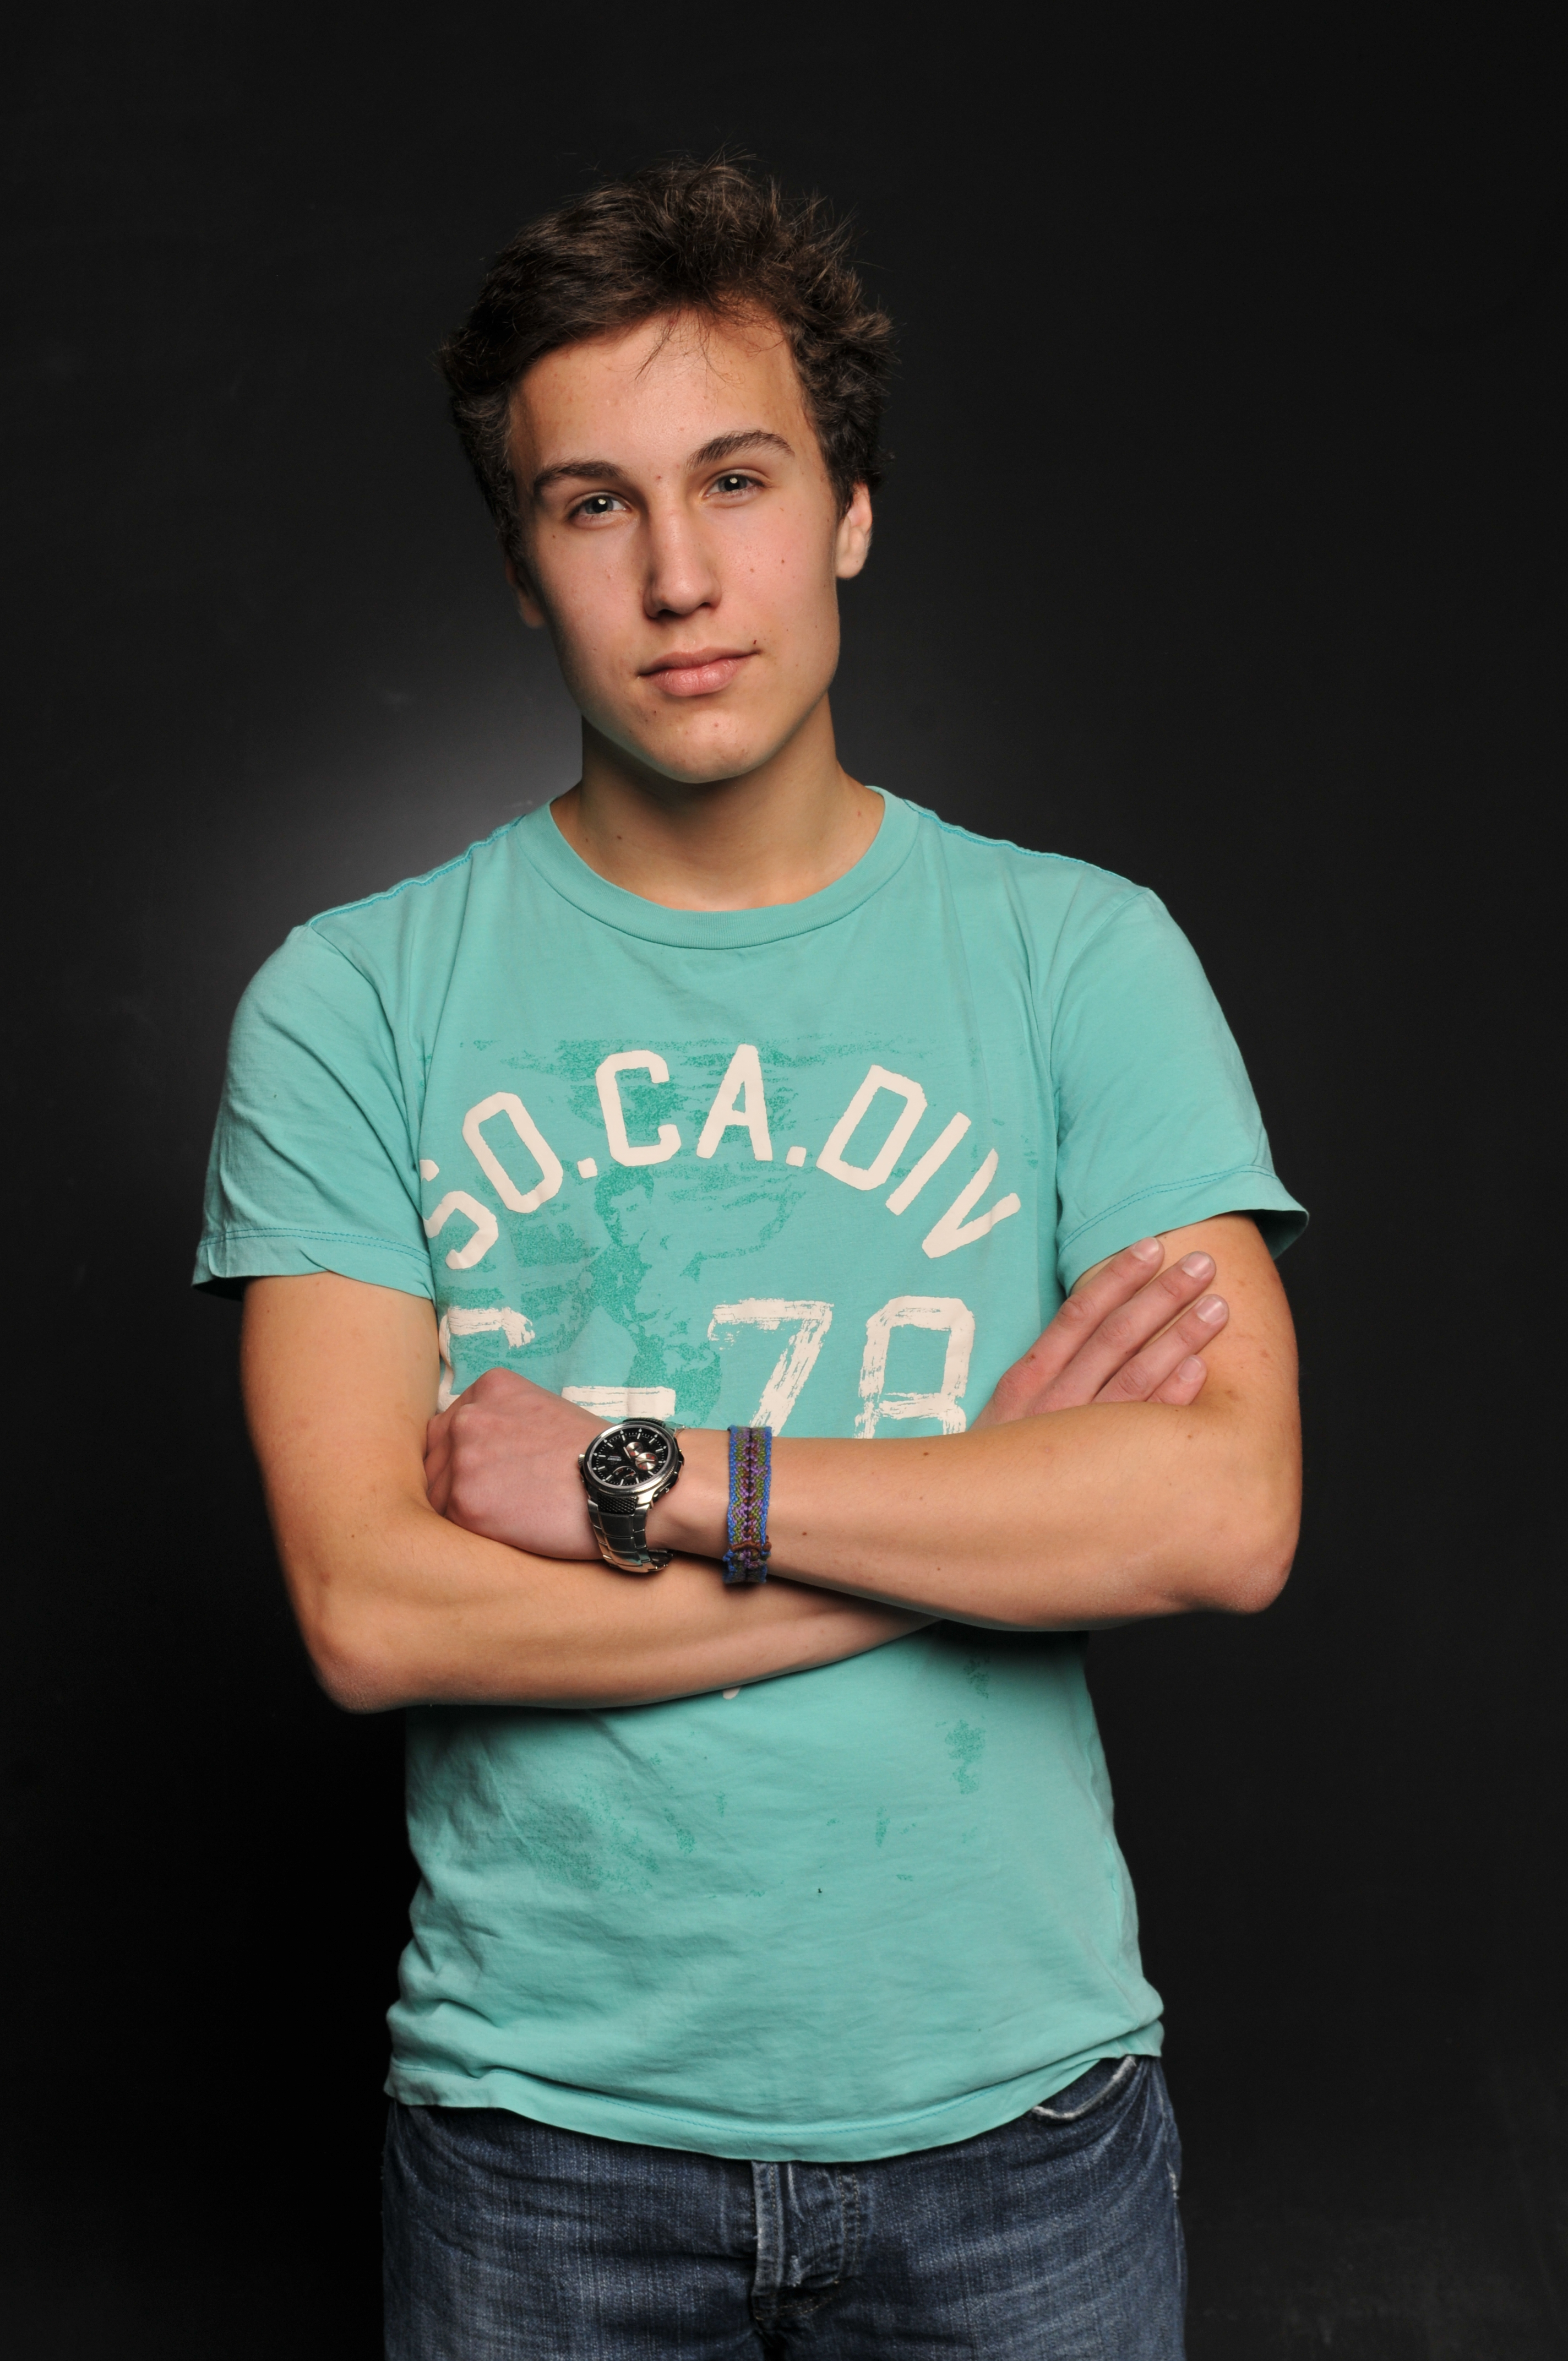
\includegraphics[scale=0.22]{1Introduction/2Our_team/images/03}}\\
	\end{minipage}
\end{figure}

\begin{figure}[H]
	\begin{minipage}[h]{0.47\linewidth}
		\center{\includegraphics[scale=0.50]{1Introduction/2Our_team/images/10}}\\
	\end{minipage}
	\hfill
	\begin{minipage}[h]{0.47\linewidth}
		Alexandr Iliasov \\
		\emph{Role in team: operator-2, decorating robot, Power Design, responsible for the bucket.\\}
		\emph{Information: 16 years old, in robotics 3 years, in FTC 2 year. \\}
		\emph{Why I chose FTC: "I choose to partipucate in the FTC, because it requiers many skills in a lot of interesting themes: physics, engineering, programming, geometry. Also, you need to work in team, argument your choise and listen others. You need find problems and solve it. All that skills you can obtain in FTC."}		
	\end{minipage}
	\vfill
\end{figure}

\begin{figure}[H]
	\begin{minipage}[h]{0.47\linewidth}
		Anton Ponikarovsky\\
		\emph{Role in team: , communication with other teams and community, reserve operator-2, responsible. \\  }
		\emph{Information: 17 years old, in robotics 3 years, in FTC 2 year. \\}
		\emph{Why I chose FTC: "I decided to join FTC because I believe that this competition is one of the most challenging of those, which are familiar to me. It requires responsibility, capability of working in team, communication with other teams, working on hardware, software and even tecnical documentation. All the experience you accumulate through doing FTC, you can apply in your future profession, if it is technical oriented."}			
	\end{minipage}
	\hfill
	\begin{minipage}[h]{0.47\linewidth}
		\center{\includegraphics[scale=0.3]{1Introduction/2Our_team/images/12}}\\
	\end{minipage}
\end{figure}

\begin{figure}[H]
	\begin{minipage}{0.47\linewidth}
		\center{\includegraphics[scale=0.22]{1Introduction/2Our_team/images/01}}\\
	\end{minipage}
	\hfill
	\begin{minipage}{0.47\linewidth}
		Andrew Nemow\\
		\emph{Role in team: drive-operator, responsible for the writing the program, responsible for debris collecting systems.\\}
		\emph{Information: 16 years old, in robotics 2 years, in FTC 1 years.\\} 
		\emph{Why I chose FTC: "When I first I attended the event FTC saw hefty metal robots, with enthusiasm and without hesitation decided that I would like to do this."}				
	\end{minipage}
	\vfill
\end{figure}

\begin{figure}[H]
	\begin{minipage}{0.47\linewidth}
		Gordei Kravzov\\
		\emph{Role in team: development strategy in the game, responsible for chassis.\\ }
		\emph{Information: 16 years old, in robotics 2 years, in FTC 1 year. \\ } 
		\emph{Why I chose FTC:"I enjoy making huge and complicated mechanisms work, that's why I chose FIRST FTC. In my opinion it's a great way to improve your skills and broaden the mind doing something that you love by the whole heart."}		
	\end{minipage}
	\hfill
	\begin{minipage}[h]{0.47\linewidth}
		\center{\includegraphics[scale=0.25]{1Introduction/2Our_team/images/11}}\\
	\end{minipage}
\end{figure}

\fillpage